Finden Sie nichtdeterministische endliche Automaten für die folgenden
Sprachen
\begin{teilaufgaben}
\item
$\{w\in\Sigma^*\,|\, |w|_{\texttt{0}}\ge 2\}$ mit
$\Sigma=\{\texttt{0},\texttt{1}\}$.
\item
$\{w\in\Sigma^*\,|\, |w|_{\texttt{0}}\le 2\}$ mit
$\Sigma=\{\texttt{0},\texttt{1}\}$.
\item
Sei $\Sigma=\{\texttt{a},\texttt{b},\texttt{c}\}$.
Ein Wort $w\in\Sigma^*$ ist genau dann in der Sprache, wenn vor jedem
Buchstaben des Wortes alle alphabetisch früheren Buchstaben vor dem Buchstaben
schon vorgekommen sind.
Es gehören also zur Sprache
\[
\texttt{aaa},\quad
\texttt{abc},\quad
\texttt{aaababc}
\]
aber nicht
\[
\texttt{ac}
\quad\text{oder}\quad
\texttt{bc}
\]
\end{teilaufgaben}

\thema{Zustandsdiagramm}
\themaL{regular}{regulär}
\thema{NEA}

\begin{loesung}
Natürlich gibt es jeweils mehrere mögliche Lösungen, nichtdeterministische
endliche Automaten sind nie eindeutig bestimmt.
\def\punkte{
	\coordinate (s) at (-2,0);
	\coordinate (q0) at (0,0);
	\coordinate (q1) at (2,0);
	\coordinate (q2) at (4,0);
	\coordinate (q3) at (6,0);
	\pfeil{(s)}{(q0)}{}
}
\def\zustand#1#2{
	\draw #1 circle[radius=0.4];
	\node at #1 {#2};
}
\def\akzeptierzustand#1#2{
	\draw #1 circle[radius=0.35];
	\zustand{#1}{#2}
}
\def\pfeil#1#2#3{
	\draw[->,shorten >= 0.4cm,shorten <= 0.4cm] #1 -- #2;
	\node at ($0.5*#1+0.5*#2$) [above] {#3};
}
\def\bogenpfeil#1#2{
	\draw[->,shorten >= 0.4cm,shorten <= 0.4cm]
		#1 to[out=60,in=120,distance=1.4cm] #1;
	\node at ($#1+(0,1.3)$) {#2};
}
\begin{teilaufgaben}
\item
\phantom{0}
\begin{center}
\begin{tikzpicture}[>=latex,thick]
\punkte
\zustand{(q0)}{$q_0$}
\zustand{(q1)}{$q_1$}
\akzeptierzustand{(q2)}{$q_2$}
\pfeil{(q0)}{(q1)}{\texttt{0}}
\pfeil{(q1)}{(q2)}{\texttt{0}}
\bogenpfeil{(q0)}{\texttt{0},\texttt{1}}
\bogenpfeil{(q1)}{\texttt{0},\texttt{1}}
\bogenpfeil{(q2)}{\texttt{0},\texttt{1}}
\end{tikzpicture}
\end{center}
\item
\phantom{0}
\begin{center}
\begin{tikzpicture}[>=latex,thick]
\punkte
\akzeptierzustand{(q0)}{$q_0$}
\akzeptierzustand{(q1)}{$q_1$}
\akzeptierzustand{(q2)}{$q_2$}
\pfeil{(q0)}{(q1)}{\texttt{0}}
\pfeil{(q1)}{(q2)}{\texttt{0}}
\bogenpfeil{(q0)}{\texttt{1}}
\bogenpfeil{(q1)}{\texttt{1}}
\bogenpfeil{(q2)}{\texttt{1}}
\end{tikzpicture}
\end{center}
\item
\phantom{0}
\begin{center}
\begin{tikzpicture}[>=latex,thick]
\punkte
\akzeptierzustand{(q0)}{$q_0$}
\akzeptierzustand{(q1)}{$q_1$}
\akzeptierzustand{(q2)}{$q_2$}
\akzeptierzustand{(q3)}{$q_3$}
\pfeil{(q0)}{(q1)}{\texttt{a}}
\pfeil{(q1)}{(q2)}{\texttt{b}}
\pfeil{(q2)}{(q3)}{\texttt{c}}
\bogenpfeil{(q1)}{\texttt{a}}
\bogenpfeil{(q2)}{\texttt{a},\texttt{b}}
\bogenpfeil{(q3)}{\texttt{a},\texttt{b},\texttt{c}}
\end{tikzpicture}
\end{center}
Obwohl alle Zustände Akzeptierzustände sind, werden nicht alle Wörter
akzeptiert.
\qedhere
\end{teilaufgaben}
\end{loesung}

